\documentclass{article}
\usepackage{graphicx} % Required for inserting images
\usepackage{outlines}
\usepackage{svg}
\usepackage{hyperref}
\usepackage{tikz}
\usetikzlibrary{positioning}

% Modernizing Radiology Workflow: Implementing PACS with RadiPush at Hargesia Group Hospital in Somaliland
% RadiPush: A Text Messaging System for Critical Radiology Findings at Hargesia Group Hospital in Somaliland
\title{RadiPush: A Prototype of Picture Archiving and Communication System (PACS) at Hargesia Group Hospital in Somaliland}
\author{Dr. Tex Li-Hsing Chi, D.D.S., Ph.D.}
\date{\today}

\begin{document}


\begin{titlepage}
%    \centering

%\begin{center}
\hspace*{-0.7cm}%
\begin{tikzpicture} % tikzfigure
%\begin{minipage}[b]{1\linewidth}

\includesvg[height=3.0cm, distort=false]{Flag_of_the_Republic_of_China.svg}
\hspace{1.4cm}
%\includesvg[width=0.17\linewidth]{TMM_logo.svg}
%\hspace{3cm}
\includesvg[height=3.0cm, distort=false]{Flag_of_Somaliland.svg}
%\captionof{Figure}{xx}
%\end{minipage}
\end{tikzpicture}
    \vspace{2cm}
    
\centering
    {\Huge\bfseries Taiwan Medical Mission in the Republic of Somaliland \\
    \par } % \\
 %   Handbook\par}
    \vspace{1.5cm}
    %\hspace{4cm} 
    {\Large \today \par}

%\end{center}

\vspace{2.0cm}
%\includesvg[height=1.0cm, distort=false]{TMWH_logo_TAIPEI_vector.svg}
\includegraphics[height=1.5cm]{TMWH_logo_TAIPEI_vector.pdf}
\includesvg[height=1.5cm, distort=false]{logo_MoHD_HGH.svg}\\
\vspace{1cm}
\includesvg[height=4cm, distort=false]{TMM_logo.svg}


\end{titlepage}



\maketitle

\section{Abstract}
Radiology reports with critical findings require timely communication to referring physicians to ensure proper patient care. However, the current system of paper printouts causes delays at Hargesia Group Hospital (HGH) in Somaliland. RadiPush is a proposed system to allow text messaging of radiology reports with critical findings directly to referring physicians' mobile phones. This prospective study will evaluate the feasibility, reliability, and physician satisfaction of using RadiPush compared to the standard paper-based system. Critical radiology reports will be sent via RadiPush and the standard system simultaneously. Outcome measures will include transmission times, physician receipt confirmation, and satisfaction surveys. We hypothesize RadiPush will provide more reliable and rapid delivery of critical radiology findings.

% new abstract
%Timely communication of critical radiology findings is essential for proper patient care. However, reliance on paper printouts causes dangerous delays at Hargesia Group Hospital (HGH) in Somaliland. RadiPush is a proposed system to automatically text message radiology reports with critical findings directly to referring physicians’ mobile phones the moment the report is finalized. RadiPush will be implemented alongside a new radiology PACS to modernize imaging workflow at HGH. This prospective pilot study will evaluate the feasibility, accuracy, reliability, and physician satisfaction of RadiPush compared to the current paper-based system over 6 months. Critical radiology reports will be delivered via simultaneous RadiPush texts and printouts. Outcome measures will include transmission times, receipt confirmation rates, diagnostic accuracy, and satisfaction surveys. We hypothesize RadiPush will provide more reliable, rapid, and accurate communication of critical results versus printouts. Findings will inform scalability and optimization of sustainable IT solutions like RadiPush to improve radiology communication and care coordination in low-resource settings.

\section{Introduction}

Taiwan Medical Mission (TMM) in the Republic of Somaliland would like to deliver a PACS project at Hargesia Groups Hospital (HGH) with the support of RadiPush and PathoPush in the radiology and pathology departments, respectively.

A picture archiving and communication system (PACS) at HGH could support telemedicine by providing remote access to medical images and reports. 
%This would allow healthcare professionals to access, view and analyze diagnostic images using a number of digital tools from any location. 
%It could also support real-time collaboration with colleagues and improve workflow for healthcare professionals.
%% A summary: 
The PACS server is the core component of the PACS architecture. It uses the DICOM standard to handle and store data about medical imaging. Several medical imaging machines, like CT scanners, MRI machines, and ultrasound machines, are linked to the PACS system. These devices make medical images in the DICOM format and send them to the PACS server so that they can be stored and retrieved.


Also connected to the PACS server are various information systems such as the hospital information system (HIS), radiology information system (RIS), and pathology information system (PIS). These systems can be integrated with the PACS server to provide a seamless flow of medical imaging data throughout the hospital.

In addition to these core components, the PACS architecture at HGH will also include support for telemedicine through teleradiology and telepathology. This allows healthcare professionals to remotely access and view medical images and reports using digital tools.

Finally, the PACS architecture at HGH will includes last-mile delivery through RadiPush and PathoPush. These sub-Projects provide an alarm system for critical diagnoses, helping healthcare professionals to quickly identify and respond to emergency or critical situations.



\section{Current Medical Images in HGH}
%%% *** why and rationale
%HGH Background: Provide information about HGH and its 
% please write two paragraphs to describe the current challenges and limitations faced by the radiology and pathology departments of HGH in terms of remote access to medical images and reports. such as HIS is available at OPD and emergency departemtn (ED), with text support only. there is only isolated images systems at the radiology and pathology departments. the current workflow: patients visit OPD, doctor prescribe CT-scan or x-ray, patients go to radiation departments. Patients bring CD-rom of DICOM and go back OPD, doctor interpret images from CD-ROM (using computer) or from printed x-ray film putting on a x-ray viewing box.   and doctor also read paper report along with CD-ROM. On pathology report, doctor take biopsy from patients during a surgery, the pathology department has pathologist doctor to make a diagnosis from pathology whole slide images. the paper report from pathologist will be brought by patient or family to doctor at OPD (the surgeon who make that biopsy). sometime patient/family will be confused from reading pathology report by their self without surgeon's explanation, such as cancer diagnosis could be a very big trouble or mis-understanding by this way. So PACS system will help to solve this major issues. medical images/reports could be transferred by system other than by patient's hands. 
The radiology and pathology departments of Hargesia Group Hospital (HGH) face a number of situations because doctors can't share medical pictures and reports. The hospital information system (HIS) is available in the outpatient department (OPD) and the emergency department (ED), but it only works with text. The image tools for radiology and pathology are separate, and the usual process for getting medical images and reports is slow and inefficient.

When a patient goes to the OPD, their doctor could inform them they need a CT scan or X-ray. They will then go to the radiology room to get the scans done. Then, they bring a CD-ROM with the DICOM images or a printed X-ray film back to the OPD. The doctor uses a computer or an X-ray viewing box to work out what these pictures are indicating. Along with the CD-ROM, the doctor also reads a paper report. For pathology reports, a specimen of tissues from the patient is taken during surgery and sent to the pathology department for study. The pathologist then makes a diagnosis based on the images of the whole slide and makes a medical report, which the patient or their family brings back to the OPD. This process can be confusing for patients and their families, especially when it comes to understanding complicated medical information like cancer diagnoses.


%%

By connecting medical images and reports between doctors, a PACS system at HGH could help solve those situations mentioned above.
PACS can help radiologists make more accurate diagnoses by making it easier for them to investigate and recognize diagnostic images. A good reporting system can also speed up the process of making reports by getting rid of the need to type patient information into apps like MS Word manually. This can help doctors provide better care to their patients.
%PACS can streamline the process of reviewing and analyzing diagnostic images. This can help radiologists to make more accurate diagnoses and report making (instead of duplicating key in of patient basic information on MS Word software) and provide better care to their patients.
This would let doctors and nurses use digital tools to access, study, and explore diagnostic images from anywhere. 
The PACS will provide remote access to medical images and reports, support real-time collaboration among healthcare professionals, and improve the current workflow of healthcare in HGH.

%RadiPush and PathoPush sub-Projects will help in an alarm system in emergency or critical situations of patients when a diagnosis reaches a threshold of danger.
RadiPush and PathoPush are parts of an overall initiative that aims to give patients an alarm system when a diagnosis hits a certain level of danger. RadiPush focuses on radiology diagnoses that fit certain critical scenarios, like tension pneumothorax, airway compromise, and cardiac tamponade. PathoPush, on the other hand, is all about finding out if someone has cancer.

By providing an alarm system for critical diagnoses, RadiPush and PathoPush can help healthcare professionals quickly identify and respond to emergency or critical situations. This can improve patient outcomes and help to save lives in situations where timely intervention is critical.

\section{Project Proposal of RadiPush}
RadiPush is a system to provide text message delivery of radiology reports with critical findings to referring physicians at Hargesia Group Hospital (HGH) in Somaliland. 
When a radiologist generates a report with critical findings, such as a pneumothorax or dissected aorta, they will designate it in the radiology information system (RIS) or a temporary gateway system to trigger an automated text message through RadiPush. 
The text will contain the patient name, key finding (e.g. "pneumothorax"), and Radiologist's contact information. It will be sent to the referring physician's mobile phone instantaneously when the PDF report is finalized. The referring doctor can then immediately contact the radiologist by phone to discuss the findings and coordinate urgent patient care. 
In addition to the text, a PDF of the report will be sent via WhatsApp. 
RadiPush aims to reduce delays and errors caused by reliance on paper printouts to communicate critical radiology results. Its impact will be evaluated by comparing transmission times, physician receipt confirmation rates, and satisfaction versus the standard paper-based system over a 6 month pilot study.


\section{Project Proposal of PACS}
%%%% PACS and DICOM
In TMM's proposal, it includes the specific needs and goals of HGH described above, as well as the benefits of implementing a PACS system with telemedicine support, and a delivery of a diagnosis report system by subprojects: RadiPush and PathoPush. 

Telemedicine, which includes teleradiology and telepathology, could be built into PACS in a native way.

PACS also has the features of RadiPush and PathoPush. In critical or emergency cases, doctors who order radiology or pathology examinations will get a text report from the short message service (SMS) of the cell phone network and a PDF report through WhatsApp software on the internet. In-depth patient care could be helped by the last-mile delivery of reports.

% 2023/06/03
We consulted with the IT specialists in Taiwan Technique Mission, which is implementing a hospital management system (HIS) in HGH to determine the best solution for our specific needs.


\section{Architecture of PACS for HGH}

The PACS architecture in HGH provides a standardized and efficient way to manage medical imaging data and ensure that it is accessible to healthcare professionals when and where it is needed.\\
The project involves the following architectures:

\begin{outline}
    \1 PACS will be installed in the radiology and pathology departments of HGH
        \2 Digital Imaging and Communications in Medicine, or DICOM, is the international standard for transmitting, storing, retrieving, printing, processing, and displaying information about medical imaging. It ensures that medical images meet quality standards and are used in most health organizations for diagnosis alongside clinical inputs. DICOM files usually include a large amount of additional data relevant to the core imaging information (pixel data which may be encoded in different ways). DICOM is essential to PACS.

        \2 PACS server: This server acts as a central repository for medical imaging data and is responsible for storing, retrieving, and transmitting DICOM files.
        \2 Connected to the PACS server are various medical imaging devices such as CT scanners, (MRI machines, future plans), and ultrasound machines. These devices generate medical images in DICOM format and transmit them to the PACS server for storage and retrieval.
        \2 Also connected to the PACS server are various desktop workstations and viewing devices (e.g., tablets and smartphones) used by healthcare professionals to access and view medical images, via 
            \3 Intranet connections
            \3 Wire or wireless connections
%These devices use specialized software to communicate with the PACS server and retrieve DICOM files for viewing.

        \2 Other systems can be integrated with the PACS server to provide a seamless flow of medical imaging data throughout HGH.
        \3 Hospital information systems (HIS) and Electronic health record (EHR) systems
        \3 Radiology information systems (RIS)
        \3 Pathology information systems (PIS)
        \3 Virtual autopsy or VIRTOPSY in Forensic Medicine. Virtual autopsy, also called postmortem imaging, is a non-invasive alternative to a traditional autopsy. It uses medical imaging techniques like computed tomography (CT) and magnetic resonance imaging (MRI) to see and record the internal structures of a dead person for forensic purposes. RIS and PIS can help with a virtual autopsy by managing and storing the medical imaging data that is made during the process. In forensic medicine, a virtual autopsy can give important information about the cause and manner of death, as well as other forensic data. It can be especially helpful when a standard autopsy can't be done or isn't wanted for religious or cultural reasons, or when the body has already started to break down. The virtual autopsy can also give more full and detailed information about the skeletal system and the major changes in the parenchyma.

%It is important to note that virtual autopsy is not intended to replace traditional autopsy, but rather to complement it by providing additional information that can aid in forensic investigations.

%Source: Conversation with Bing, 30/05/2023(1) The approach of virtual autopsy (VIRTOPSY) by ... - ScienceDirect. https://www.sciencedirect.com/science/article/pii/S2666225620300105 Accessed 30/05/2023.
%(2) A Practical Guide to Virtual Autopsy: Why, When and How. https://www.sciencedirect.com/science/article/pii/S0887217118300945 Accessed 30/05/2023.
%(3) Radiology in Forensic Medicine - Springer. https://link.springer.com/book/10.1007/978-3-319-96737-0 Accessed 30/05/2023.
        % the PIS (Pathology information system) automates samples, images, and reports and progressively incorporates PI (Pathology informatics), D-PATH (digital pathology), e-PATH (electronic pathology), PPH (Patho-pharmacology), virtual autopsy, and in general all types of translational research in the PMIS (pathology management information system).
        
\1 Telemedicine
    \2 DICOM images from ultrasound machines, or point-of-care ultrasound (POCUS) devices, could be sent from one place to another.
    
    \2 Teleradiology is the electronic transmission of DICOM images from one location to another. It has various applications, such as case referrals, consultation services, and education. In this project, we propose to use teleradiology to provide case consultation between Somaliland and Taiwan.

    \2 Telepathology is the electronic transmission of pathological images, usually derived from microscopic slide scanners, from one location to another. A DICOM converter should be applied to produce DICOM images from pathological images (e.g., MIRAX) which are acquired by microscopic slide scanners. It has various applications, such as case referrals, immunohistochemistry (IHC) services, and education. In this project, we propose to use telepathology to provide case consultation and IHC services between Somaliland and Taiwan. A workflow of telepathology includes:
%This includes images from various medical imaging modalities such as radiology, ultrasound, and pathology.


	\3 A pathologist in HGH, Somaliland, will share whole slide images through Vision Assist App.
 %will use the Vision Assist app to scan and export whole slide images of pathology in MIRAX format (one of the OpenSlide standard formats) from tissue samples obtained during surgery or biopsy. Then it could be converted as DICOM and uploaded in PACS.
    
%    \3 Dr. Omar will upload the images to PACS and share them with a pathologist in Taipei.
     %, Taiwan, who will review them using QuPath software (\url{https://qupath.readthedocs.io/en/0.4/docs/intro/installation.html}). Alternatively, the Taipei pathologist can use their preferred software viewer if it can read MIRAX files.

    \3 The Hargeisa and the Taipei pathologists will communicate via Webex Meetings (\url{https://www.webex.com/video-conferencing}), a free and secure online tool for video conferencing that allows screen sharing and annotation. They will do bi-weekly teleconsultations of digital pathology for referring cases and training on the job. They will discuss the diagnosis and treatment options based on the images and the clinical information. This is meant to assist in building up the pathology profession in Somaliland and make it easy for pathologists from Taiwan and Somaliland to work together.
    
    \3 If immunohistochemistry (IHC) is needed for precision diagnosis, Dr. Omar will send formalin-fixed paraffin-embedded (FFPE) tissue blocks to Taipei via DHL Medical Express, a reliable and fast courier service for medical specimens. The Taipei pathologist will perform the appropriate IHC process and share the results. The patient will be responsible for paying for IHC services and DHL fees.
% (\url{https://www.dhl.com/global-en/home/our-divisions/express/industry-sectors/life-sciences-and-healthcare.html})

\1 Last-mile delivery
    \2 PACS server is accessed by computer/tablet in HGH (reports and images)
    \2 RadiPush and PathoPush: an alarm system for critical diagnoses. It can help healthcare professionals quickly identify and respond to emergency or critical situations. This can improve patient outcomes and help to save lives in situations where timely intervention is critical.
    
        \3 RadiPush (reports through SMS): to give patients an alarm system when a diagnosis hits a certain level of danger. RadiPush focuses on radiology diagnoses that fit certain critical scenarios, like tension pneumothorax, airway compromise, and cardiac tamponade. 
        Deep learning model of (large language models) LLM should also help in the reporting system with a "co-pilot" of radiologist. 

        \3 PathoPush (reports through SMS): to give patients an alarm system when a diagnosis hits a certain level of danger. PathoPush is all about finding out if someone has cancer.

 
\end{outline}

\clearpage
%%%%%%%%%%%%%%%

% RadiPush in Hargeisa Group Hospital


% tikzpicture
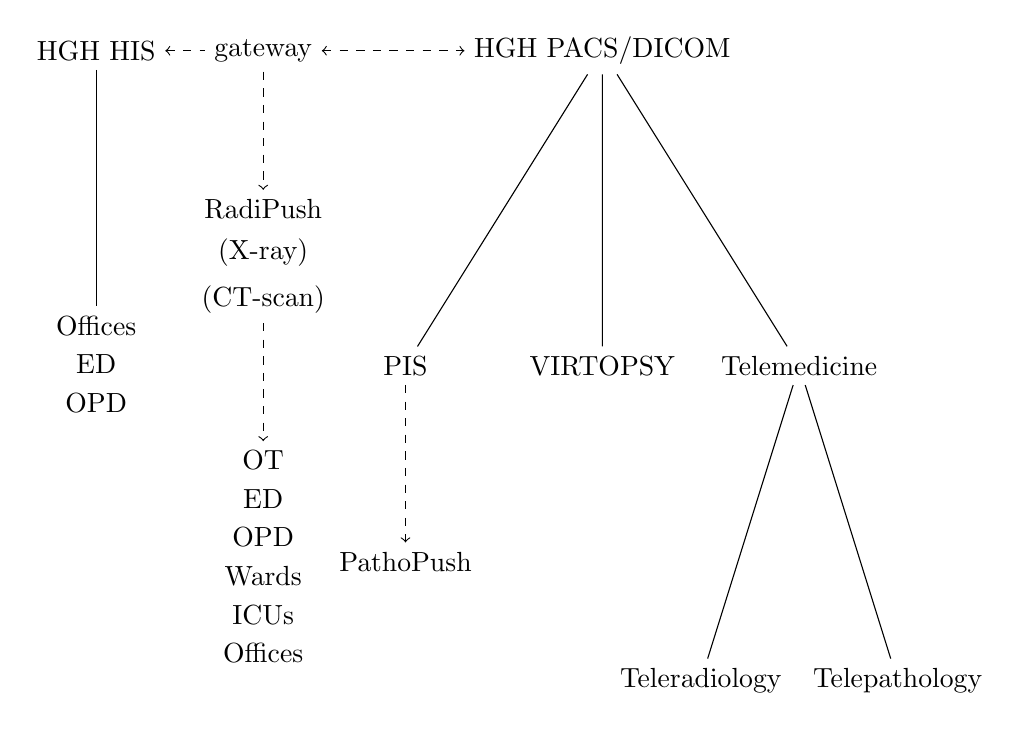
\begin{tikzpicture}[
    level 1/.style={sibling distance=25mm, level distance=40mm},
    level 2/.style={sibling distance=25mm},
    level 3/.style={sibling distance=20mm, level distance=30mm}]
%    level 4/.style={sibling distance=20mm, level distance=30mm},
%    level 5/.style={level distance=30mm},
%    level 6/.style={level distance=30mm},
%    level 7/.style={level distance=30mm},
%    level 8/.style={level distance=30mm}]
\node (his) {HGH HIS};
\node[below=30mm of his] (ot1) {Offices};
\draw (his) -- (ot1);
\node[below=0mm of ot1] (ed1) {ED};
\node[below=0mm of ed1] (opd1) {OPD};
%\node[below=0mm of opd1] (wards1) {Wards};
%\node[below=0mm of wards1] (icus1) {ICUs};
%\node[below=0mm of icus1] (offices1) {Offices};
%\node[below=0mm of offices1] (radiPush1) {RadiPush};

\node[right=5mm of his] (tex) {gateway};
%    child {node (radi){Radiology:}};
\node[below=15mm of tex] (radp) {RadiPush};
\draw[dashed, ->] (tex) -- (radp);
    \node[below=0mm of radp] (xr) {(X-ray)};
    \node[below=0mm of xr] (ct) {(CT-scan)};

%        child {node {CT}}
%        child {node {X-ray}}};

\node[right=38mm of his] (pacs) {HGH PACS/DICOM} % ---
%    child {node {PACS Server}
%        child {node {CT}}
%        child {node {X-ray}}}
%    child {node (ris) {RIS}}
%        child[grow=down, edge from parent/.style={draw}] {node (ot) {OT}}
%        child[grow=down, edge from parent/.style={draw=none}] {node {ED}}
%        child[grow=down, edge from parent/.style={draw=none}] {node {OPD}}
%        child[grow=down, edge from parent/.style={draw=none}] {node {Wards}}
%        child[grow=down, edge from parent/.style={draw=none}] {node {ICUs}}
%        child[grow=down, edge from parent/.style={draw=none}] {node {Offices}}
%        child[grow=down, edge from parent/.style={draw=none}] {node {RadiPush}}}
    child {node (pis) {PIS}}
%        child {node {PathoPush}}}
    %child {node {HIS}}
    child {node {VIRTOPSY}}
    child {node {Telemedicine}
        child {node {Teleradiology}}
        child {node {Telepathology}}};
       % child {node {Ultrasound}}};
%\node[left=of pacs] (his) {HIS};
%\node[right=3cm of pacs] (his) {HIS};
%\draw (his) edge[<->] (tex);
\draw [dashed, <-] (his) -- (tex);
\draw [dashed, <->] (tex) -- (pacs);

\node[below=15mm of ct] (ot) {OT};
\draw[dashed, ->] (ct) -- (ot);
%\draw (ris) -- (ot);
\node[below=0mm of ot] (ed) {ED};
\node[below=0mm of ed] (opd) {OPD};
\node[below=0mm of opd] (wards) {Wards};
\node[below=0mm of wards] (icus) {ICUs};
\node[below=0mm of icus] (offices) {Offices};
%\node[below=0mm of offices] (radiPush) {RadiPush};

\node[below=20mm of pis] (pathopush) {PathoPush};
\draw[dashed, ->] (pis) -- (pathopush);






%\node [below of = Telemedicine] {Teleradiology}
%    child {node {Teleradiology}}
%    child {node {Telepathology}}
%    child {node {Ultrasound}};
%\node [below of = HGH PACS] {Last-mile Delivery}
%    child {node {RadiPush}}
%    child {node {PathoPush}};
%\node [below of = {PACS Server}] {DICOM compliance}
\end{tikzpicture}
% You can also customize the diagram by changing the values of sibling distance and level in the code.

The hierarchy diagram of PACS (DICOM compliance), and RadiPush gateway: It includes PACS server, medical imaging, CT scanners, ultrasound machines, hospital information system, radiology information system (RIS), pathology information system (PIS), virtual autopsy (VIRTOPSY), telemedicine, teleradiology, telepathology, RadiPush, and PathoPush.
Due to the vast spread of departments and system stability, the HGH intranet system should ideally be connected over a fiberoptic network.
However, it could be delayed until year 2025.
Before the implementation of PACS in Hargeisa Group Hospital, a RadiPush or PathoPush will be conducted through a gateway, as a provisional RIS or PIS, respectively.
(OT: operation theatre, ED: emergency department, OPD: outpatient department, ICU: intensive care unit)
%%%%%%%%%%%%%%
\clearpage

\section{Implementation Plan}
\begin{outline}
    \1 the steps involved in implementing the PACS at HGH
        \2 plan on 2023: RadiPush and PathoPush, pilot study
        \2 plan on 2024: fiber optic network
        \2 plan on 2025: PACS
    \1 the resources and costs required for implementation
    \1 Potential challenges or limitations and how they will be addressed
\end{outline}

\section{Conclusion}

%Summarize the benefits of implementing a PACS system with telemedicine support at HGH
%Reiterate the goals of TMM in delivering this project

%Here is a draft conclusion incorporating the use of large language models like GPT-4 as a "co-pilot" for radiologists with RadiPush and PACS:

%Conclusion:


%Here is a rewrite of that paragraph:

The implementation of a PACS system with teleradiology and telepathology support at Hargesia Group Hospital has immense potential to modernize workflows. The ability to instantly access medical images and data across departments will enable rapid diagnoses, improved collaboration between staff, and efficient coordination of patient care. Specifically, the integration of the RadiPush and PathoPush critical findings alert systems into the radiology and pathology workflows will be transformative. Automated text messaging of urgent radiology and pathology results directly to referring clinicians' phones can accelerate the communication of actionable test findings. This could lead to lifesaving interventions in critical situations where each minute counts. 
Overall, PACS with integrated telemedicine and last-mile reporting solutions will bring Hargesia Group Hospital to the digital medical era with improved diagnostics, enhanced teamwork, and potentially better patient outcomes.
%Also, a PACS system can make it easier to look at and analyze diagnostic images, which can help radiologists make more correct diagnoses and give their patients better care.


Additionally, integration of large language models such as GPT-4 as a "co-pilot" to assist radiologists has exciting possibilities. These models can be trained on radiology text and imaging to provide radiologists with real-time support during image interpretation and reporting. They can suggest differential diagnoses for validation by the radiologist, as well as provide evidence-based recommendations for further imaging or clinical management. 
%Studies have shown such AI assistance can improve radiologist productivity and reduce reporting errors.


%%
The Taiwan Medical Mission (TMM) will consult with the IT specialists in Taiwan Technique Mission to determine the best solution for their needs.
The project will be evaluated the feasibility, accuracy, reliability, and efficiency of PACS for case discussion and consultation service and its impact on patient outcomes, healthcare professionals’ satisfaction, and healthcare costs.
%TMM wants to improve the quality of care at HGH by installing a PACS system with telemedicine support. 
%TMM plans to help HGH give better care to its patients by giving doctors and nurses online access to medical images and reports and making it easier for them to work together.

%The projects will also contribute to advancing telemedicine as an emerging form of advanced healthcare in Somaliland.
In conclusion, implementing PACS, RadiPush, and LLMs like GPT-4 can modernize radiology at Hargesia Group Hospital for more accurate and timely diagnosis. This will lead to improved clinical outcomes and patient care through faster communication of critical results and emerging AI support tools. Careful evaluation of costs, training requirements, and clinical integration will be important to successfully translate these technologies' benefits into practice.


\end{document}


%%%% spared

\section{Draft Schedule}
An ENT campaign (e.g., operation for Tonsillitis) in Hargeisa, Somaliland, in August 2023:
\begin{outline}

	\1 (Briefing) On August 12 (Saturday), Dr. Hung will arrive one day ago and meet Dr. Omar, Dr. Hersi in Hargeisa, and the other local authorities and health officials to discuss the objectives and logistics of the campaign. They will also visit the Hargeisa Group Hospital (HGH) and inspect the facilities and equipment available for the surgery. They will review the list of patients Dr. Hersi screened and collected in July and select the most suitable candidates for the operation (a maximal of 40 patients).
	\1 (Surgery at HGH OT: August 14, 15) 
        \2 On August 14 (Monday) and August 15 (Tuesday), Dr. Hung and Hersi will perform the surgery on the selected patients at HGH with the assistance of local medical staff. They will also provide post-operative care and instructions to the patients and their families. They will monitor the recovery and outcomes of the surgery and document any complications or challenges. 
	\1 (Surgery or Debriefing)
        \2 On August 16 (Wednesday), they will also conduct a debriefing session with the local health authorities and HGH staff to share their feedback and recommendations for future campaigns.
\end{outline}


\section{Suggested Surgery}
Which kind of ENT surgery? by literature review:

Based on the web search results, some of the suggested ENT surgeries or diseases according to health statistics in Somaliland (or Somalia) are:

\begin{outline}

\1 *Tonsillitis, inflammation of the tonsils that can cause sore throat and fever.
\1 Cancer affecting the oral buccal mucosa, or lip in stage I without neck nodal disease clinically.
\1 Otosclerosis, a condition of the middle ear that causes hearing loss.
\1 Otitis media with effusion, also known as glue ear, in which the middle ear becomes blocked with fluid.
\1 Nasal polyps, benign growths in the nose that can cause obstruction and infection.

These are some of the common ENT problems that affect the population of Somaliland, especially children and elderly people. They may require surgical intervention or medical management depending on the severity and type of the condition.
\end{outline}


\section{Reference}
(1) Interpreting the Lancet surgical indicators in Somaliland: a cross-sectional study. https://bmjopen.bmj.com/content/10/12/e042968 Accessed 11/05/2023.
(2) ENT Department | Somali Sudanese specialized hospital. ENT Department | Somali Sudanese specialized hospital (ssshospital.so) Accessed 11/05/2023.